AzuDICI\footnote{You can find the latest implementation of AzuDICI at
  \url{https://github.com/leoferres/AzuDICI}} is a standard CDCL
solver based on \pling, {\tt barcelogic} and {\tt miraXT}, built with
the aim of finding out whether or not sharing information among
threads (particularly the clauses database) helps avoid the
performance degradation that can be seen in Figure \ref{fig:decay}.

In particular, AzuDICI implements binary implication lists for the
propagation with binary clauses, and the two-watched literals scheme
for unit propagation \cite{} with clauses of more than two
literals. AzuDICI also implements the 1-UIP algorithm for conflict
analysis \ref{}, the lemma simplification algorithm used in {\tt
  PicoSAT}, Luby restarts \cite{}, a policy for lemma cleaning that
keeps only binary and ternary lemmas, and more than four-literal
lemmas that have participated in a conflict since the last
cleanup. Finally, AzuDICI also incorporates the EVSIDS heuristic for
branching literal decisions \cite{}.

\begin{figure}[tp]
  \centering
  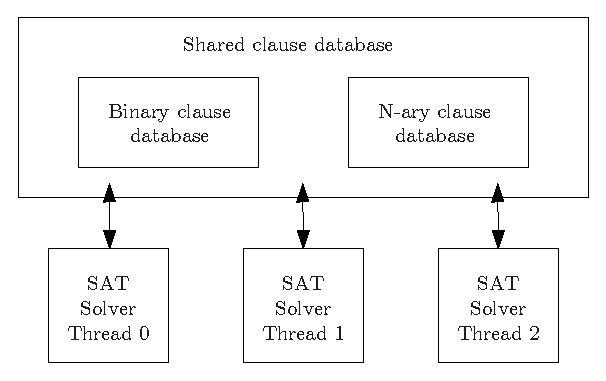
\includegraphics[scale=0.7]{AzuDICI_database}
  \caption{Shared clause database among threads.}
  \label{fig:azu database}
\end{figure}

In order to allow for comparison, we made several versions of AzuDICI.
AzuDICI-shared-all is a version which shares all clauses between
threads. It has a shared clause database which includes unitary
clauses, binary clauses and n-ary clauses (clauses with more than
two literals). Figure \ref{fig:azu database}
shows how threads share the clause database. Each thread has access
to the same physical clauses and they do not require synchronization
with each other.
Because binary implication lists are simple data structures that do
not keep track of watched literals, it is easy to share binary clauses
between threads without hindering the performance of propagation
or any other task each sequential worker thread performs. This is not
the case for the n-ary clause database. The two-watched-literal
scheme requires to make changes to the clause in order to identify
the literals being watched at one given instant (for example, place
both literals first in the clause). Since many threads will be
accessing the same clauses, these changes to the clause are not
feasible to share n-ary clauses. Instead, we have used a similar 
approach as used in
{\tt miraXT}, where each thread keeps track of the literals being
watched in each clause. Figure \ref{fig:azu design} is a
schematization of how each thread worker relates with the n-ary
clause database. Each SAT solver thread has a vector of pointers
to thread clauses called \textit{watches}, and each literal present
in the SAT problem has a position associated in this watches vector.
A thread clause has two watched literals (WL0 and WL1), two
pointers to another thread clause (NW0 and NW1) and a pointer to
an actual n-ary clause in the n-ary clause database. W0 and W1 keep
track of the literals being watched by the thread for a given n-ary
clause. NW0 and NW1 point to the next thread clauses that are also 
watching WL0 and WL1 respectively.

\begin{figure}[tp]
  \centering
  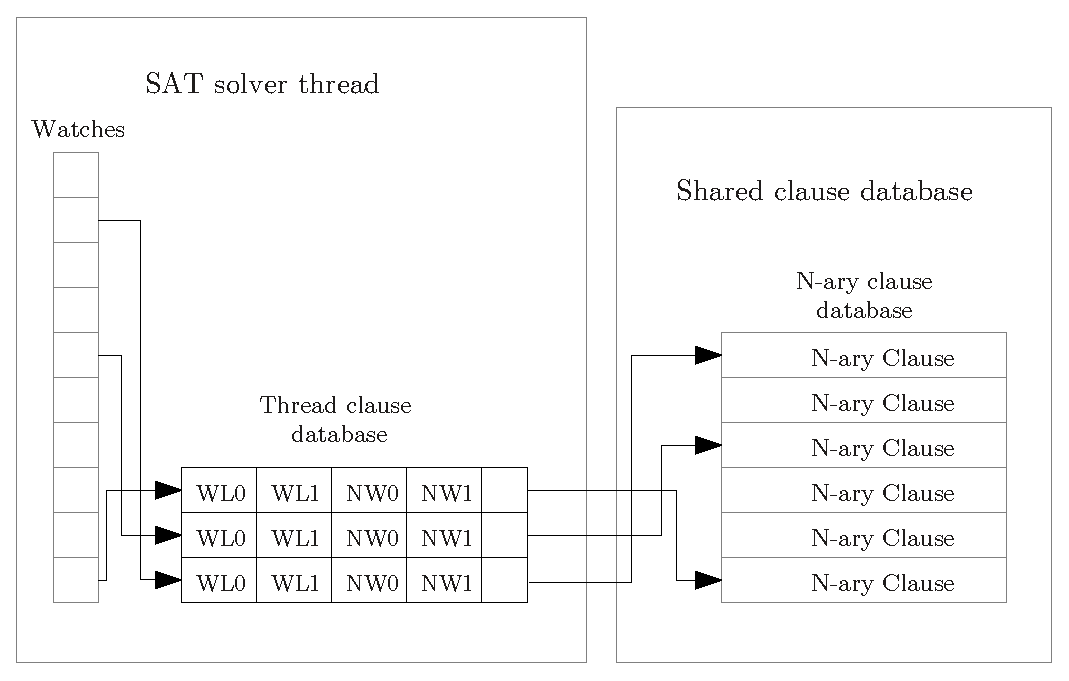
\includegraphics[scale=0.6]{AzuDICI_design}
  \caption{The thread clause database and n-ary clause database}
  \label{fig:azu design}
\end{figure}

As sharing n-ary clauses requires to make some changes to the
implementation of the propagation scheme of the two-watched-literals,
we also made the AzuDICI-shared-binaries version, which only shares
the binary clause database. With this version we aim to find out
if the drawbacks of sharing n-ary clauses, because we have to keep
track of each watched literal in each thread, surpass the benefits.
The AzuDICI-shared-none version doesn't share any clause and it's
just a group of independent solvers running in parallel, each with
its own clause database.

It is important to note that in order to make this comparison of
different solver versions objective, we have forced them all to make
the exact same search, so that the differences in performance we
observe will not be due to the search path each version takes.
For the same reason, all threads in each version of the solver will
also make the same search. We would not want an instance of a
solver performing better just because an additional thread found
a better search path.

Regarding thread safety of the solver versions which share clauses,
we added some locks to ensure the correctness of the information
being shared. The locks are only used to avoid two different threads
inserting clauses to a same clause database at the same time,
because the chance that this event occurs is so low, in practice
there is no significant contention between threads.

%%% Local Variables: 
%%% mode: latex
%%% TeX-master: "sat"
%%% End: 
